
The goal of the advanced IMP utilization for OZG is to improve upon the solution presented in chapter 4 while allowing it to be modify and replace large portions of the existing system architecture. 

\section{IMP Solution Integration}

\subfile{13-imp_solution_integration}

\section{Technological Integration}

\subfile{14-technological_integration}

\subsection{Solution Evaluation}

\begin{center}
    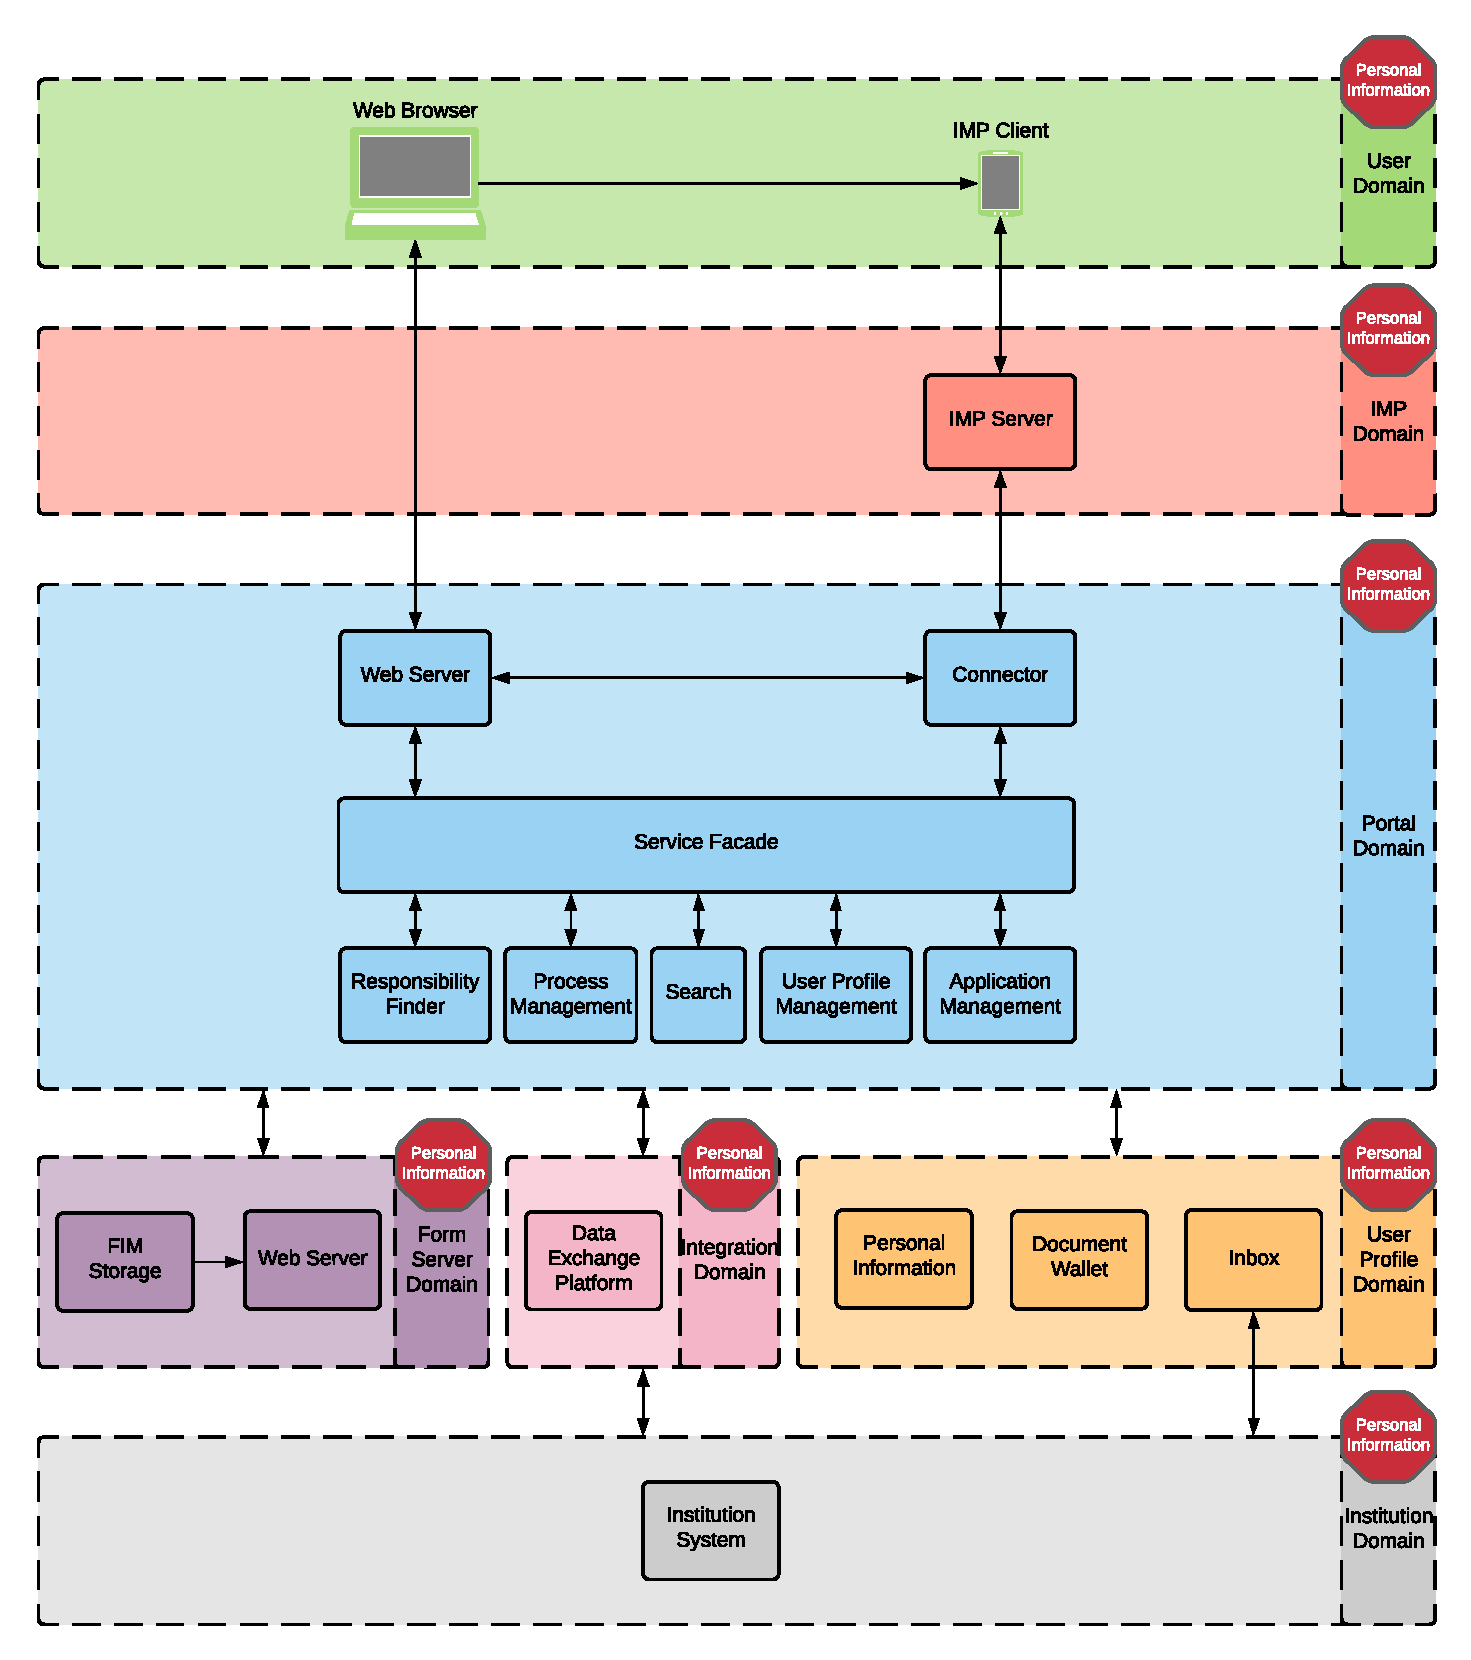
\includegraphics[scale=0.6]{Diagrams/Integration Architecture 2/Personal Information Existing Architecture.pdf}
\end{center}

\begin{center}
    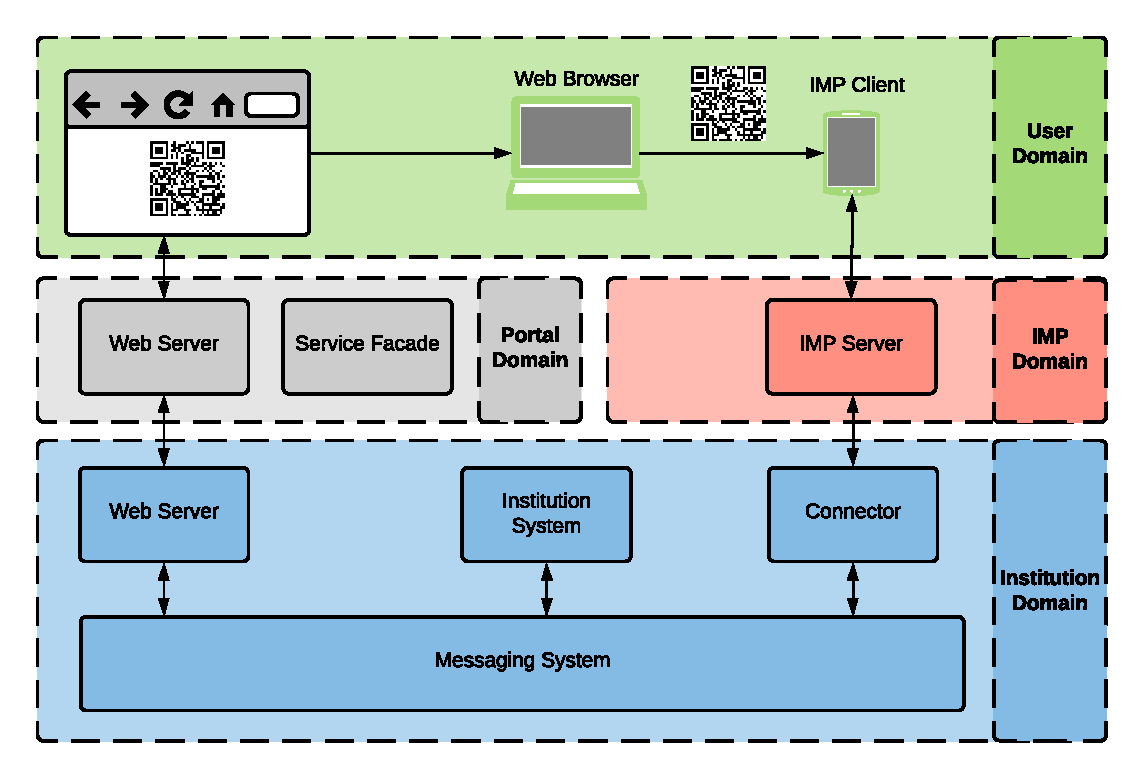
\includegraphics[scale=0.6]{Diagrams/Integration Architecture 2/Overview.pdf}
\end{center}


\begin{itemize}
    
    \item Integration aufbauend auf erster oder ersetzend??
    
    \item Messaging architektur aus 1 genau so applizierbar in advanced integration
    
    \item im stil der overview der integrationen auch das connection diagram des OZG systems beschreiben. User Domain, Portal Domain, FIM Domain, Institution Domain, Data Exchange Domain
    
    \item basic use case umsetzen durch IMP trotz ablösen von 3 vorher existierenden domänen
    
    \item in diagrammen aufzeigen wo persönliche daten verarbeitet werden
    
    \item datenverabeitung vergleich zwischen diagrammen
    
    \item offen ob man andere domänen abschaltet (übergangszeit anlassen)
    
    \item benefit of module for each application type is, that the processing of applications with different legitimations is fully seperated and in the future new apllication types can be added without touching exisitng modules
\end{itemize}